\section{Is it Time to Replace CNNs with Transformers for Medical Images?}

\subsection*{Ссылка} \url{https://arxiv.org/abs/2108.09038}
\subsection*{Введение}
В течение последних лет сверточные нейронные сети (СНС)
являлись лидирующим методом в автоматической медицинской 
диагностике. Однако, недавно появившиеся vision transformers
(ViT), являются достойной альтернативной для СНС, достигая 
схожих уровней производительности, обладая некоторыми интересными свойствами,
которые могут быть полезными в задачах распознавания медицинских 
изображений. В данной работе исследуется возможность замены 
сверточных нейронных сетей трансформерами ViT в задачах 
медицинской автоматизации и какие плюсы это принесет. 
\subsection*{Основная идея}
Для того, чтобы получить ответ на поставленный вопрос, авторы
провели серию экспериментов, сравнивая ViT и СНС при одинаковых
условиях, минимально изменяя гиперпараметры. Чтобы обеспечить 
чистоту эксперимента, были выбраны ResNet50, как представитель СНС 
и DeiT-S, как представитель ViT, так как они сравнимы по 
количеству параметров, затратам памяти и вычислительным мощностям.
Инициализация СНС проводилась по трем стратегиям: (1) инициализация весов 
случайными значениями; (2) трансферное обучение (transfer learning) с 
с использованиям весов, предобученных на ImageNet; (3) self-supervised предобучение 
на целевом датасете, после инициализации как в пункте (2). Каждый эксперимент
повторялся пять раз и выбирались результаты с самой высокой точностью
на валидационном множестве.
\subsection*{Данные}
APTOS 2019, ISIC 2019, CBIS-DDSM
\subsection*{Результаты}
При случайной инициализации весов СНС превосходит ViT. Такая 
закономерность выявлена при обучении на всех трех датасетах.
Однако, при использовании весов, предобученных на ImageNet, 
разрыв между производительностью СНС и ViT в данной задаче 
сходит почти на нет.  Таким образом, можно заключить:
\begin{itemize}
    \item ViT проигрывает СНС при случайной инициализации 
    весов и обучении с нуля;
    \item Трансферное обучение устраняет разрыв в производительности
    между ViT и СНС;
    \item Наилучший результат получен при подходе self-supervised+
    pre-training+ fine-tuning, при котором ViT слегка превосходит СНС.
\end{itemize}

\\

\begin{minipage}{1.0\linewidth}
    \begin{center}
        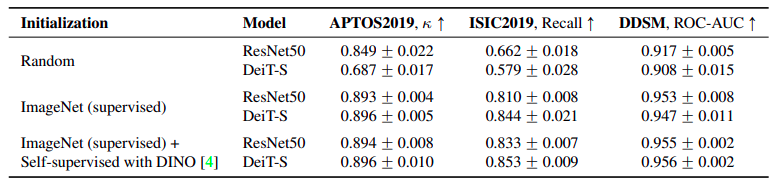
\includegraphics[scale=0.5]{ann11_res.png} \\
        \caption{\scriptsize{Сравнение результатов предсказания СНС и ViT в разрезе различных стратегий инициализации весов 
        на медицинских изображениях.}}
    \end{center}
    
\end{minipage}

\begin{minipage}{1.0\linewidth}
    \begin{center}
        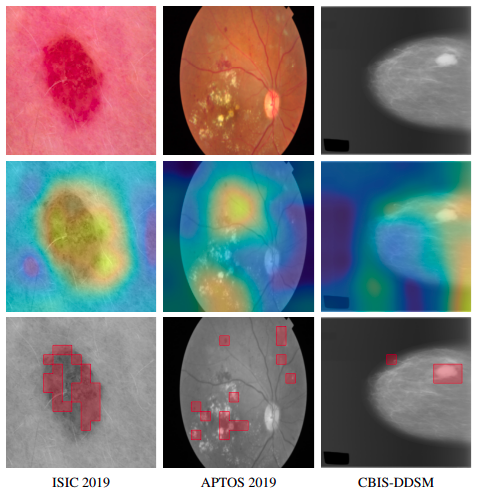
\includegraphics[scale=0.4]{ann11_res2.png} \\
        \caption{\scriptsize{Сравнение карт значимости (saliency maps) изображений из трех датасетов. В каждой колонке 
        представлены оригинальное изображение, визуализация ResNet50 Grad-CAM saliency map и карты внимания (attention map) DEIT-S.}}
    \end{center}
    
\end{minipage}

\subsection*{Заключение}
В данной работе проводится анализ возможности замены сверточных
нейронных сетей трансформерами (ViT) в задачах распознавания
медицинских изображений. Показано, что ViT по качеству сравнима 
с СНС и может быть использована как альтернативный уже существующим метод.